\documentclass[11pt, a4paper]{article} %tamaño mínimo de letra 11pto.
\usepackage{url} %Para incluir páginas web como referencia
\usepackage[dvipsnames]{xcolor} %Para colores raros que quiera usar.

\usepackage{amsfonts} %Para poder poner letras bonitas de números naturales etc.
\usepackage{tikz} % Para hacer recuadros para las fórmulas
\usepackage{mdframed} % Para hacer cuadritos
\usepackage{graphicx} % Para incluir imágenes
\usepackage{xcolor} % Para algunos colores
\usepackage{amsmath} % Para matemáticas
\usepackage{multirow} % Para poder hacer celdas combinadas en las tablas
\usepackage{float} % Para que se coloque la tabla donde realmente has puesto el código
\usepackage{hyperref} % Para que funcionen los links
\usepackage[spanish]{babel} % Español 
\usepackage[utf8]{inputenc} % Para poder poner tildes
\usepackage{vmargin} % Para modificar los márgenes
\newtheorem{Teorema}{Teorema} %Para generar teoremas
\setmargins{2.5cm}{1.5cm}{16.5cm}{23.42cm}{10pt}{1cm}{0pt}{2cm}
%margen izquierdo, superior, anchura del texto, altura del texto, altura de los encabezados, espacio entre el texto y los encabezados, altura del pie de página, espacio entre el texto y el pie de página
\mdfdefinestyle{theoremstyle}{%
linecolor=blue!40,linewidth=2pt,%
frametitlerule=true,%
frametitlebackgroundcolor=gray!20,
innertopmargin=\topskip,
}
%\mdtheorem[style=theoremstyle]{definition}{Definición}
\newtheorem{definicion}{Definición}[section]
\newtheorem{proposicion}{Proposición}[section]

\newtheorem{propiedad}{Propiedad}[section]

\newtheorem{ejemplo}{Ejemplo}[section]

\begin{document}

%%%%%%Portada%%%%%%%
\begin{titlepage}
\centering
{ \bfseries \Large UNIVERSIDAD COMPLUTENSE DE MADRID}
\vspace{0.5cm}

{\bfseries  \Large FACULTAD DE CIENCIAS FÍSICAS} 
\vspace{1cm}

{\large DEPARTAMENTO DE ARQUITECTURA DE COMPUTADORES Y AUTOMÁTICA}
\vspace{0.8cm}

%%%%Logo Complutense%%%%%
{
\includegraphics[width=0.35\textwidth]{images/logo_UCM}} %Para ajustar la portada a una sola página se puede reducir el tamaño del logo
\vspace{0.8cm}

{\bfseries \Large TRABAJO DE FIN DE GRADO}
\vspace{2cm}

{\Large Código de TFG:  DACYA-11 } \vspace{5mm}

{\Large Generación de energía con una turbina eólica flotante}\vspace{5mm}

{\Large Energy generation with a floating offshore wind turbine}\vspace{5mm}

{\Large Supervisor: Matilde Santos Peña}\vspace{20mm} 

{\bfseries \LARGE José Antonio Fernández López}\vspace{5mm} 

{\large Grado en Ingeniería Electrónica de Comunicaciones}\vspace{5mm} 

{\large Curso académico 2021-2022}\vspace{5mm} 

{\large Convocatoria junio}\vspace{5mm} 

\end{titlepage}


\newpage

%{\bfseries \large [Título extendido del TFG (si procede)] }\vspace{10mm} 

{\bfseries \large Resumen:} \vspace{5mm}


Esto es una prueba para probar el formato del Resumen.
\vspace{1cm}

\begin{otherlanguage}{english}
{\bfseries \large Abstract: }\vspace{5mm}


This is a test to prove the abstract's layout.
\vspace{1cm}
\end{otherlanguage}

%[\Large\textbf{Nota}: el título extendido (si procede), el resumen y el abstract deben estar en una misma página y su extensión no debe superar una página. Tamaño mínimo 11pto ]\\

%{\Large\textbf{Extensión máxima 50 páginas sin contar portada ni resumen (sí se incluye índice, introducción, conclusiones y bibliografía}}
\newpage
\tableofcontents
\section{Introducción}

\subsection{Motivación}

Cuál es el problema que vas a tratar
Utilidad del estudio
Aplicación

\subsection{Objetivos}
El objetivo principal de este trabajo es...
Los objetivos específicos son:
\begin{itemize}
    \item Estudiar la fuerza de torsión en la pala de un aerogenerador
    \item Encontrar el modelo matemático de las fuerzas
\end{itemize}

\subsection{Estructura de la memoria}

\subsection{Asignaturas relacionadas}
\section{Desarrollo teórico de la fuerza de torsión en una pala de una turbina eólica}

\subsection{Descripción de la pala del aerogenerador y sus parámetros}

En esta sección se va a describir la pala del aerogenerador y los parámetros necesarios para determinar los efectos que produce la torsión en nuestra obtención de energía. En primer lugar definición e idea general de una pala, desarrollo trigonométrico para el cálculo de la línea de cuerda,... \colorbox{orange}{RELLENAR}


Se determina que la pala de la turbina eólica es un \textbf{trapecio} cuya representación simplificada se muestra en la Figura \ref{fig:pala_simp}. \\\\




\begin{figure}[H]
    \centering
    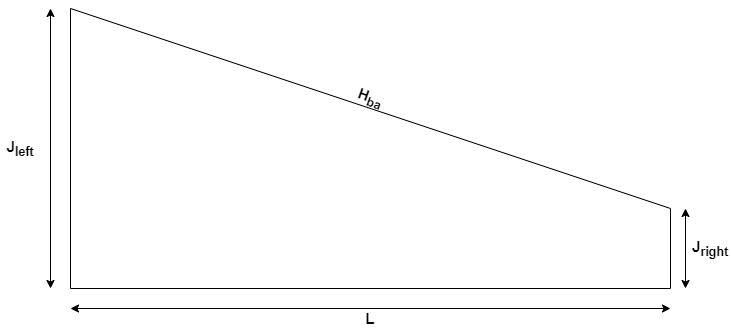
\includegraphics[width=1\textwidth]{images/pala simple.drawio.png}
    \caption{Representación de una pala de turbina eólica}
    \label{fig:pala_simp}
\end{figure}


Lo siguiente que debe tenerse presente es que se necesita también una representación de la pala como la que se puede observar en la Figura \ref{fig:pala_simp}. Esta está dividida en segmentos de igual largo para poder comprender el desarrollo que se realizará simulando una torsión, en la cual se girarán los segmentos un cierto ángulo los unos de los otros.

\begin{figure}[H]
    \centering
    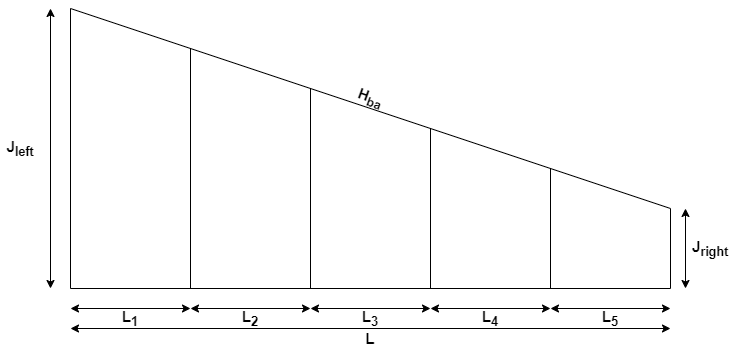
\includegraphics[width=1\textwidth]{images/pala simple segmentada.drawio.png}
    \caption{Representación de una pala de turbina eólica dividida en segmentos}
    \label{fig:pala_dividida}
\end{figure}

Por simplicidad, la pala se dividirá únicamente en $N$ segmentos, en este trabajo se utilizará $N=5$. Aunque se mantenga este valor durante el trabajo se asociará a una variable en caso de que se quieran hacer pruebas mediante simulación en MATLAB más adelante. \\\\
    

Se define la variable $L$ como la longitud de la pala (ver Figura \ref{fig:pala_simp}). Como puede observarse, cada uno de los segmentos de la Figura \ref{fig:pala_dividida} tendrá una longitud de segmento $L_i = \dfrac{L}{N} (m)$ donde $i \in \{1,...,N\}$.\\

Como se puede observar en la Figura \ref{fig:pala_dividida} cada segmento tiene una altura variable, esto se debe a la forma real de las palas, cuanto más cerca del buje de la turbina, mayor es el área del segmento. La altura en el centro de estos segmentos, conocida como \textit{chord line} (que se denotará como $c_i$ con $i \in \{1, ...,N\}$) o línea de cuerda, se determinará fijando los valores de la longitud de la pala $L$, la longitud del buje (que se denotará por $J_{left}$) y la longitud de la punta (que se denotará por $J_{right}$). Una vez establecidos estos valores se puede dar paso al desarrollo matemático de la pala.\\

\begin{figure}[H]
    \centering
    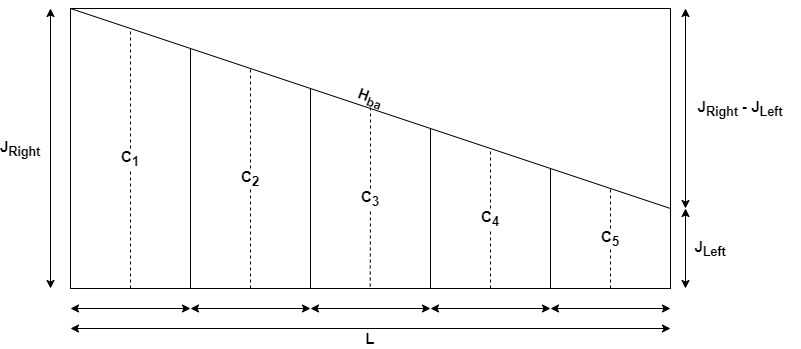
\includegraphics[width=1\textwidth]{images/planteo chord line.drawio.png}
    \caption{Representación parametrizada de la pala de una turbina eólica}
    
    \label{fig:pala_desarrollo_chord}
\end{figure}

Para el cálculo de la línea de cuerda se requiere la realización de un desarrollo trigonométrico. \\

En base a la Figura \ref{fig:pala_desarrollo_chord} se puede deducir que
$J_{rigth} = \dfrac{J_{left}}{D} (m)$ donde D es el factor de reducción de alto de pala y $D \in \mathbb{Q+}$. Además, se debe cumplir que $J_{left} > D$.\\

El factor reductor $D$ procede de la naturaleza del análisis y cómo se ha afrontado el estudio simplificado de una pala de aerogenerador. Si bien es cierto que se pudo realizar de una manera aún más simple haciendo que la pala fuese un rectángulo, se prefirió abordar con una forma trapezoidal. Así, los tres parámetros $J_{left}$, $J_{rigth}$ y $L$ se calculan en función del valor de $D$. Esto permite hacer los cálculos con una relación entre la longitud del buje $J_{left}$ y de la punta $J_{right}$ de las palas de la turbina eólica, esto además permite que el problema sea más general. \\

Se define el valor de la hipotenusa del borde de arrastre $H_{ba}$ mediante el Teorema de Pitágoras, ya que se trata de un triángulo rectángulo (en azul en la Figura \ref{fig:pala_calculo_phi}). Así, se tiene:
\begin{equation}
H_{ba} = \sqrt{(J_{left} - J_{right})^{2} + L^{2}}
\label{def_hipotenusa_pala}
\end{equation}


\begin{figure}[H]
    \centering
    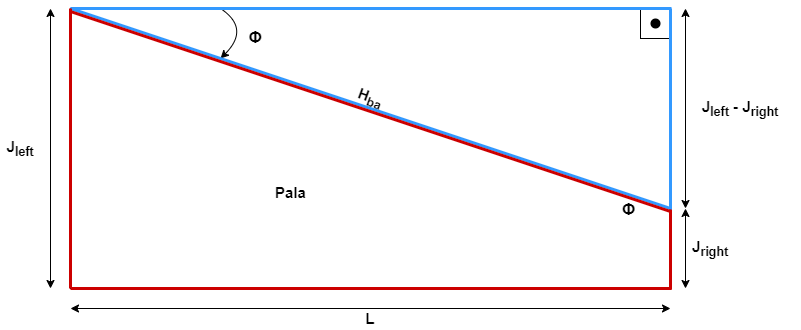
\includegraphics[width=0.9\textwidth]{images/triangulo sacar phi.png}
    \caption{Pala de la turbina en amarillo y triángulo usado para el cálculo de $\Phi$ en azul}
    
    \label{fig:pala_calculo_phi}
\end{figure}

A continuación, se debe obtener el ángulo de la línea del borde de arrastre de la pala de la turbina eólica $\Phi$, para así conocer cómo decrece el valor de $H_{ba}$.
En base a la Figura \ref{fig:pala_calculo_phi} se puede calcular de tres formas distintas mediante la trigonometría el valor del ángulo $\Phi$:
\begin{equation}
 \Phi = \arcsin{\left(\dfrac{c_{left} - c_{right}}{H_{ba}}\right)} (^{\circ})
\label{def_angulo_phi_1}
\end{equation}

\begin{equation}
 \Phi = \arccos{\left(\dfrac{L}{H_{ba}}\right)} (^{\circ})
\label{def_angulo_phi_2}
\end{equation}

\begin{equation}
 \Phi = \arctan{\left(\dfrac{\sin{\left(\dfrac{c_{left} - c_{right}}{H_{ba}}\right)}}{\cos{\left(\dfrac{L}{H_{ba}}\right)}}\right)} (^{\circ}) 
\label{def_angulo_phi_3}
\end{equation}

\colorbox{orange}{HACERLO CON TALES}


\\

% Para calcular las \textit{líneas de cuerda} $c$, se aíslan los trapecios más pequeños de los que se han obtenido todos los datos menos el valor de su base menor que se tendrá que calcular, siendo este equivalente a $c$.\\

% \begin{equation}
% Variables necesarias para el cálculo de las líneas de cuerda.

%  altura_i = \dfrac{(2i - 1) \cdot L}{2N}
%  diagonal_i = \dfrac{(2i - 1) \cdot H_{bf}}{2N}

% Donde,
% \centering
% $altura_i$ := Longitud de la pala fragmentada para el cálculo de la línea de cuerda y $diagonal_i$ := Longitud de la hipotenusa del borde de fuga fragmentada para el cálculo de la línea de cuerda.
% \label{def_variables_fragmentadas}
% \end{equation}

% Por último y una vez definido todo lo necesario, se pasa al cálculo mediante el cual se obtiene el valor de todas y cada una de las $líneas \text{ } de \text{ } cuerda$ de la pala con la que se está trabajando.

% \begin{equation}
% Primero se obtiene la diferencia mediante Pitágoras entre la base mayor y la menor, definida como $x_i$, después la resta de la base mayor y esta diferencia.

%  x_i = \sqrt{diagonal_i^{2} - altura_i^{2}}

%  c_i = c_{left_i} - x_i 
% \label{def_chord_line}
% \end{equation}

% La siguiente figura, ilustra el ejemplo en el que para las definiciones \ref{def_variables_fragmentadas} y \ref{def_chord_line} el valor de $i$ es igual a 3. Obteniendo así $c_3$. En verde el trapecio y en magenta el triángulo del que restamos el cateto a la base mayor del trapecio.

% \begin{figure}[H]
%     \centering
%     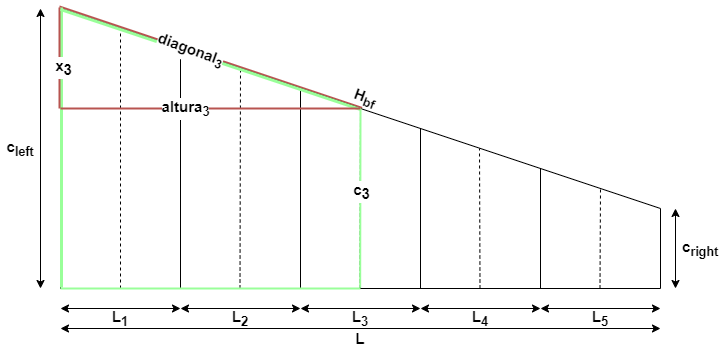
\includegraphics[width=0.9\textwidth]{images/Trapecio calculo x.png}
%     \caption{Representación gráfica del cálculo realizado en las definiciones \ref{def_variables_fragmentadas} y \ref{def_chord_line}}
% \end{figure}


% Una vez se ha obtenido el valor buscado $c_i$, se deberá definir todos los laterales de los segmentos de la pala, para así poder operar con ellos en pos de conseguir el área de cada uno de ellos. Esto ya fue desarrollado en el artículo \cite{armenta2021predictive}, pero en aquel caso fue usado para comprobar el error que suponía usar un rectángulo en vez de una pala simplificada. En este caso se parte directamente de la pala simplificada para evitar correcciones de errores mas adelante y porque el cálculo que se debe realizar con respecto a la obtención de energía no es tan profundo y complicado como en el artículo \cite{armenta2021predictive}. Además remarcar que para las deducciones y cálculos anteriores se bebió de este desarrollo.


% \begin{equation}
% En base a esta representación esquemática y mediante relaciones trigonométricas obtuvieron:
%  c_{left_i} = c_i + (\dfrac{L_i}{2}) \tan \varPhi
%  c_{right_i} = c_i - (\dfrac{L_i}{2}) \tan \varPhi
% \label{def:laterales_segmento}
% \end{equation}

% Al igual que se deduce en el artículo \cite{armenta2021predictive}, con los datos obtenidos de los laterales de cada segmento, se puede trabajar con una forma de trapecio y encontrar el área de los segmentos que se definieron en la Figura \ref{fig:pala_dividida}.\\

% Aparte, con esta definición se ve que en la Figura \ref{fig:pala_desarrollo_chord} los valores de $c_{left_i}$ y de $c_{right_i}$ que se observan, realmente serían equivalentes a $c_{left_1}$ y a $c_{right_5}$, respectivamente. Estos son definidos a priori debido a su importancia para caracterizar la pala de manera correcta y con las dimensiones que el usuario desee.

% \begin{equation}
% Se determina el área de los segmentos:
%  s_{i} = \dfrac{(c_{left_i} + c_{right_i})}{2N} \cdot L_i 
% Donde,
% \centering $s_i$ := Área del segmento.
% \label{def:area_segmentos}
% \end{equation}


A continuación se supone que los segmentos están ensartados por una línea imaginaria que ayudará al estudio de la torsión mediante giros de los segmentos alrededor suya. \\

Esta línea imaginaria pasará por el centro de masas de todos los segmentos. Delineando rectas en cada segmento desde una esquina a la contraria se genera un punto en el centro del segmento en el que estas rectas se cortan, siendo este punto el llamado centro de masas. Además, si se traza una línea que una el punto central de las rectas $J_{left}$ y $J_{right}$, esta recta pasará por los centros de masa de cada uno de los segmentos.\\

Cuando se ha obtenido esta recta imaginaria, se puede determinar lo que se denotará como $brazo$ que se corresponde con la longitud desde el punto central del buje $J_{left}$ hasta la línea de cuerda $c_{i}$ del segmento $i$, siendo este punto además el centro de masas del segmento $i$.


    \begin{figure}[H]
    \centering
    \includegraphics[width=1\textwidth]{images/explicación brazo.png}
    \caption{Representación de los brazos de la pala}
    \label{fig:exp_brazo}
    
\end{figure}

El brazo viene definido por la resta de las mitades de los lados de la pala. Una vez se tiene la recta que pasa por los centros de masa se determina el valor de cada uno de los brazos.
\begin{equation}
cateto \text{ } buje = \dfrac{J_{left}}{2} - \dfrac{J_{right}}{2} \hspace{7pt} (m)
\end{equation}

\begin{equation}
R \text{ } brazo = \sqrt{cateto \text{ } buje^{2} + L^{2}} \hspace{7pt} (m)
\end{equation}

\begin{equation}
brazo_i = \dfrac{(2i -1) \cdot R \text{ } brazo}{2N} \hspace{7pt} (m)
\end{equation}
Donde, $cateto \text{ } buje$ := Medida de buje o $J_{left}$ reducida para su utilización en la obtención del brazo, $R \text{ } brazo$ := Recta completa del brazo antes de dividirla dependiendo del segmento y $brazo_i$ := Distancia entre el centro de $J_{Left}$ y el centro de masas del segmento correspondiente.

\subsection{Análisis del volumen de la pala}
\label{section:volumen_pala}

Una vez definida la geometría en dos dimensiones de la pala del aerogenerador se puede añadir una nueva dimensión al análisis. En la Figura \ref{fig:analisis_volumen} se puede observar una representación adaptada para este trabajo de la pala de un aerogenerador en tres dimensiones.

    \begin{figure}[H]
    \centering
    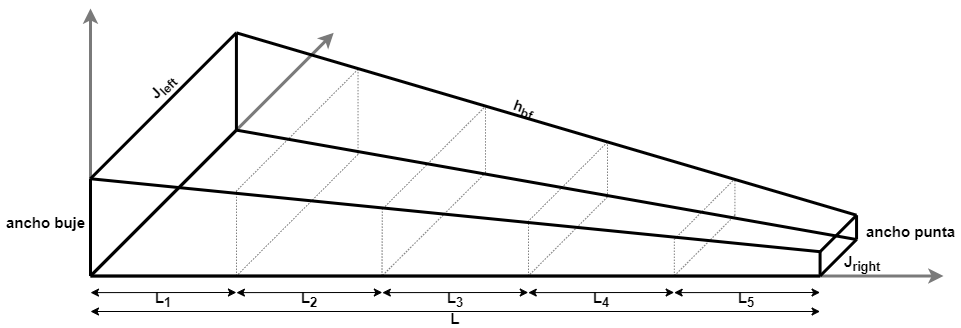
\includegraphics[width=1\textwidth]{images/pala 3d segmentada enorme.png}
    \caption{Representación gráfica de la pala segmentada en 3 dimensiones}
    \label{fig:analisis_volumen}
    \end{figure}



Mediante la observación de la figura \ref{fig:analisis_volumen} se puede averiguar lo siguiente: \\\\\\\\

\colorbox{Orange}{ \Huge Aquí va un desarrollo con otra figura, la del ancho}

\begin{equation}
Donde, recta \text{ } decrecimiento_i = \dfrac{( i \cdot \sqrt{L^2 + (ancho \text{ } punta - ancho \text{ } buje)^2)}}{N} \hspace{7pt} (m)
\end{equation}

Siendo, $ancho \text{ } buje$ y $ancho  \text{ } punta$ $\in \mathbb{Q+}$, $ancho \text{ } buje > ancho \text{ } punta$, $recta \text{ } decrecimiento_i $ := línea de disminución de la parte superior ancho de la pala dividida para cada segmento,  $ancho \text{ } punta$ := amplitud de la pala del aerogenerador en la zona más estrecha o punta y $ancho \text{ } buje$ := amplitud de la pala del aerogenerador en la zona más ancha o buje.\\


Tal y como se presentó en la Figura \ref{fig:pala_calculo_phi}, la variable $x_i$ sirvió de apoyo para calcular las reducciones de tamaño de las líneas de cuerda al ir restando el resultado a la variable $c_left_{i}$. Esto mismo ocurre para el ancho de la pala. En esta ocasión además, se necesitará una segunda variable.\\


Las variables de apoyo son las siguientes:
\begin{equation}
 z_i = \sqrt{ recta \text{ } decrecimiento_i^2 - (L_i \cdot i )^2} \hspace{7pt} (m)
 \end{equation}
 \begin{equation}
 b_i =  \left\{\begin{matrix}
0 \hspace{33pt} Sí \hspace{7pt} i = 1\\ 
z_i  \hspace{30pt} Sí \hspace{7pt}  i > 1
\end{matrix}\right
\end{equation}

Donde, $z_i$ := variable de apoyo para el cálculo del área de las secciones trapezoides correspondientes al corte de los segmentos, en este caso de las bases menores,  $b_i$ := segunda variable de apoyo pero en este caso sirve para las bases mayores.\\


Se obtiene el ancho de las bases de los troncos trapezoidales y se calculan las áreas de las bases:
\begin{equation}
 ancho \text{ } bases \text{ } menores_i = ancho \text{ } buje - z_i \hspace{7pt} (m)
 \end{equation}
 \begin{equation}
 ancho \text{ } bases \text{ } mayores_i = ancho \text{ } buje - b_i \hspace{7pt} (m)
\end{equation}
\begin{equation}
 area \text{ } bases \text{ } menores_i = ancho \text{ } bases \text{ } menores_i \cdot {c_{right}}_i \hspace{7pt} (m^2)
 \end{equation}
\begin{equation}
 area \text{ } bases \text{ } mayores_i = ancho \text{ } bases \text{ } mayores_i \cdot {c_{left}}_i \hspace{7pt} (m^2)
\end{equation}

Donde, $ancho \text{ } bases \text{ } mayores_i$ := Ancho de las bases trapezoidales de mayor tamaño con las que se calculará el volumen del tronco o frustum de cada uno de los segmentos,  $ancho \text{ } bases \text{ } menores_i$ := Ancho de las bases trapezoidales de menor tamaño con las que se calculará el volumen del tronco o frustum de cada uno de los segmentos, $ area \text{ } base \text{ } mayor_i $ := zonas trapezoidales que sirven de base mayor para el cálculo del frustum de cada segmento y $ area \text{ } base \text{ } menorr_i $ := zonas trapezoidales que sirven de base menor para el cálculo del frustum de cada segmento.\\


Con todo lo necesario para el cálculo del volumen de la pala del aerogenerador se procede a ello. Se va a realizar de dos maneras; completo y segmentado. El segmentado es necesario debido al desarrollo que se ha ido realizando y que se va a seguir durante todo el trabajo, y el completo se usará para comparación y demostración junto al segmentado para comprobar la precisión de los cálculos.\\

El volumen de la pala de una turbina eólica es definido mediante las siguientes ecuaciones:
\begin{equation}
    \begin{split}
        volumen \text{ } frustum_i = & \dfrac{L_i}{3} \cdot (area \text{ } bases \text{ } mayores_i + area \text{ } bases \text{ } menores_i \\
        & + \sqrt{area \text{ } bases \text{ } mayores_i \cdot area \text{ } bases \text{ } menores_i}) \hspace{7pt} (m^3)
    \end{split}
\end{equation}

\begin{equation}
 volumen \text{ } frustum_{total} = \sum_{i}^{N}volumen \text{ } frustum_i \hspace{7pt} (m^3)
\end{equation}

\begin{equation}
 area \text{ } base_{punta} = ancho \text{ } punta * J_{right} \hspace{7pt} (m^2)
 \end{equation}

 \begin{equation}
 area \text{ } base_{buje} = ancho \text{ } buje * J_{left} \hspace{7pt} (m^2)
 \end{equation}
 
 \begin{equation}
    \begin{split}
        volumen \text{ } frustum_{completo} = & \dfrac{L}{3} \cdot ( area \text{ } base_{punta} + area \text{ }  base_{buje}\\
        & + \sqrt{area \text{ } base_{punta} \cdot area \text{ } base_{buje}}) \hspace{7pt} (m^3) 
    \end{split}
 \end{equation}

Donde, $ volumen \text{ } frustum_i $ := tamaño de cada uno de los segmentos del tronco de pirámide de la pala del aerogenerador, $ volumen \text{ } frustum_{total} $ := tamaño absoluto de la pala del aerogenerador, $area \text{ } base_{punta}$ := zona trapezoidal de mayor tamaño usada para el cálculo del volumen del frustum, $area \text{ } base_{punta}$ := zona trapezoidal de menor tamaño usada para el cálculo del volumen del frustum y $ volumen \text{ } frustum_{completo} $ := tamaño integro de la pala del aerogenerador.\\


Teniendo los cálculos del volumen de la pala del aerogenerador se pueden estudiar a continuación los efectos que producen las simplificaciones que se han realizado para la obtención de energía.


\subsection{Estudio del torque sin ángulo de cabeceo}
\label{section:torque_pala_horizontal}
%Tomando una pala con una forma real se puede observar que se produce cierto giro de las palas del aerogenerador. En esta situación no se presenta cabeceo, es decir, el viento tiene un ángulo de ataque paralelo con la pala de la turbina eólica. \\

Tomando una pala con forma real, en una situación en la que no se presenta cabeceo, en la que está incidiendo un viento con ángulo de ataque paralelo a la pala se puede observar un giro de las palas del aerogenerador.

Al estar la pala real más redondeada por la parte superior y teniendo mayor volumen que la parte inferior y mediante el principio de Bernoulli la parte superior presenta un mayor recorrido que la inferior, y con ello una velocidad de viento mayor y por tanto una menor presión. \\

Este efecto produce un gradiente de presión y por ello una fuerza de sustentación. Debido la no simetría de las palas del aerogenerador como se muestra en la Figura \ref{fig:corte_transversal_pala}. \\

    \begin{figure}[H]
    \centering
    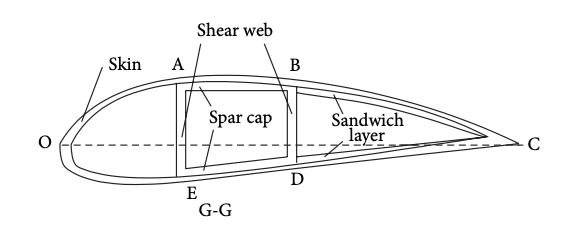
\includegraphics[width=1\textwidth]{images/Cross secction pala articulo.png}
    \caption{Corte transversal de una pala (Ver Artículo \cite{Zheng2014})}
    \label{fig:corte_transversal_pala}
    \end{figure}


Debido a este fenómeno se va a trabajar con una pala simplificada (ver la Figura \ref{fig:analisis_volumen}) que simplificará cálculos. \\



\subsection{Estudio del torque con ángulo de cabeceo}
\label{section:torque_giro_inicial}

El ángulo $ \theta_1 $ es el \textit{ángulo de cabeceo} que sufrirán todos y cada uno de los segmentos que son paralelos al plano horizontal, desde el cual se presenta el viento que incidirá en la pala.\\


En esta sección se estudiará qué ocurre en término de fuerzas, torque y momento cuando se gira toda la pala únicamente el ángulo de cabeceo $ \theta_1 $. \\


Al inclinar odos los segmentos un ángulo $ \theta_1 $ se genera la situación en la que el viento incide en el centro del segmento con el mismo ángulo con el que se inclina la pala (ver Figura \ref{fig:dibujo_angulo_ataque}). \\

\begin{figure}[H]
    \centering
    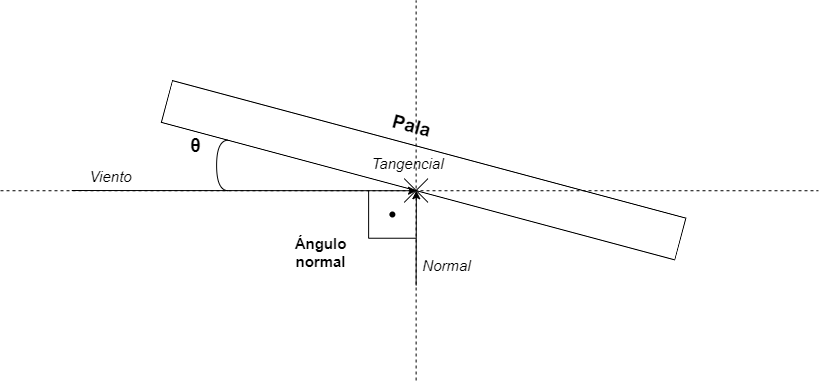
\includegraphics[width=1\textwidth]{images/dibujo fuerzas.drawio.png}
    \caption{Ángulo de ataque del viento con respecto a la pala y descomposición de vectores de fuerzas}
    
    \label{fig:dibujo_fuerzas}
\end{figure}

La fuerza del viento que incide en la pala se puede descomponer en dos, la tangencial y la normal. \\

El vector fuerza normal es perpendicular al ángulo de ataque del viento, mientras que el vector fuerza tangencial recorre de manera paralela la línea central de la pala.

 La fuerza normal viene definida por la siguiente expresión:
 \begin{equation}
   f \text{ } normal_i = F \text{ } viento_i \cdot \sin{\theta_1} \hspace{7pt} (N)
 \label{def:fuerza_normal}
 \end{equation}
 Donde, $F \text{ } viento$ := Fuerza generada por el viento en cada segmento de la pala y $f \text{ } normal$ := Fuerza perpendicular al viento, generada por el choque de este con la pala de la turbina eólica.\\


La componente paralela a la pala, que se ha definido como tangencial se obviará debido a que no genera momento de torsión o torque.\\
  
El momento de giro o torque se define como:
  \begin{equation}
  torque_0 = f \text{ } normal_i \times brazo \hspace{7pt} (N \cdot m)
  \label{def:torque_inicial}
 \end{equation}
 Donde, $torque_0$ := Momento de fuerza de giro solo con ángulo de cabeceo.\\


El $torque_0$ es el producto vectorial entre la $fuerza  \text{ }perpendicular \text{ } o \text{ } normal$ y el $brazo$. Pero estas dos variables son perpendiculares la una a la otra, es por ello que esa expresión es el producto algebraico de las variables, dando lugar a:
 
 
  \begin{equation}
  torque_{0_i} = f \text{ } normal_i \cdot brazo_i \hspace{7pt} (N \cdot m)
 \label{def:torque_algebraico_inicial}
 \end{equation}
 
 La suma de los torques es torque global.
 \begin{equation}
  torque \text{ } global_0 \text{ } = \sum_{i=1}^{N} torque_0_{i} \hspace{7pt} (N \cdot m)
\label{def:torque_global}
\end{equation}
 
 
La fuerza del viento para el rotor completo es:
 \begin{equation}
  F \text{ } viento_i = \dfrac{1}{2} \text{ } \rho \cdot area \text{ } rotor \cdot u^2 \cdot coeficiente \text{ } sustentación \hspace{7pt} (N)
   \end{equation}
   
  \begin{equation}
  area \text{ } rotor = \dfrac{\pi}{4} \cdot diametro \text{ } rotor^2 \hspace{7pt} (m^2) 
  \end{equation}
  
  \begin{equation}
  diametro \text{ } rotor = 2 \cdot L \hspace{7pt} (m)
 \end{equation}
 Donde, $\rho := 1.225 \text{ } \dfrac{Kg}{m^3}$, $u$ := velocidad del viento, $diametro \text{ } rotor $ := superficie abarcada por la pala en caso de realizar un giro completo, $area \text{ } rotor$ := superficie del círculo que dibuja el giro de las palas y $coeficiente \text{ } sustentación$ := número usado en la modelación y sus dependencias complejas de forma, inclinación y algunas condiciones de flujo en la sustentación (Ver Página web \cite{Hall2021}).
 
 
 %El coeficiente de sustentación es un número que los aerodinámicos usan para modelar todas las dependencias complejas de forma, inclinación y algunas condiciones de flujo en la sustentación. Esta ecuación es simplemente un reordenamiento de la ecuación de sustentación donde resolvemos el coeficiente de sustentación en términos de las otras variables. El coeficiente de sustentación Cl es igual a la sustentación L dividida por la cantidad: densidad r por la mitad de la velocidad V al cuadrado por el área del ala A.





 
 \subsection{Estudio del torque con ángulo de cabeceo y torsión de la pala}
\label{section:torque_giro_torsion}

La única diferencia entre este apartado y el anterior es el ángulo de giro de los segmentos. Anteriormente, se vió como todos los segmentos giraban un determinado \textit{ángulo de cabeceo}, pero ahora el ángulo que se girarán vendrá dado por:

Dados un ángulo inicial de giro $\theta_1 $ y una variación de giro constante (o no) $\Delta_\theta$, se define el ángulo de torsión de cada segmento como:
\begin{equation}
\theta_i = \theta_{i-1} + \Delta_\theta \hspace{7pt} (^{\circ})
\label{def:theta_cte}
\end{equation}
Donde, $i \in segmento \wedge (i > 1)$\\


Como se menciona, la variación $\Delta_\theta$ puede que no sea constante y entonces:
\begin{equation}
\theta_i = \theta_{i-1} + \Delta_{\theta_{i}}  \hspace{7pt} (^{\circ})
\label{def:theta_nocte}
\end{equation}
Donde, $i \in segmento \wedge (i > 1)$\\

La fuerza normal se define como:
\begin{equation}
   f \text{ } normal_i = F \text{ } viento_i \cdot \sin{\theta_i} \hspace{7pt} (N)
  \label{def:fuerza_normal_torsion}
 \end{equation}

El resto de fórmulas no varían debido a que no dependen del ángulo $\theta_i$. En el caso del \textit{torque global} la suma de torques nos aportará un conjunto de valores diferentes y que servirán como estudio.

  \begin{equation}
  torque_{1_i} = f \text{ } normal_i \cdot brazo_i \cdot \cos{\Delta_{\theta_{i}}} \hspace{7pt} (N \cdot m)
 \label{def:torque_algebraico_torsion}
 \end{equation}
 
Donde, $ \cos{\Delta_{\theta_{i}}} $ puede presentar una pequeña variación en el valor del torque. Este coseno representa el área efectiva donde se está aplicando la $ f \text{ } normal $, es decir, el área de la totalidad del segmento de la pala si fuera observada desde arriba en un plano XY. Esto se debe a que cuanto más se torsione el segmento, menos parte será visible.\\

Por último, la suma de los torques con un giro inicial es entonces:
\begin{equation}
  torque \text{ } global_1 \text{ } = \sum_{i=1}^{N} torque_{1_i} \hspace{7pt} (N \cdot m)
 \label{def:torque_global_1}
\end{equation}
Donde, $torque \text{ } global_1$ := Suma de torque de los N segmentos.





















\subsection{Cálculo de la potencia del sistema}
\label{section:pot_sistema}
 
 Una vez se tiene todo lo necesario para el cálculo del torque, se puede pasar al cálculo de la potencia. Esta es la variable más importante, cuanta mayor cantidad de energía se genere, mejor, aunque existe un límite directamente relacionado con las limitaciones técnicas y físicas que presentan las turbinas eólicas. \\
 
 
  La potencia del sistema con un ángulo de cabeceo se define como:
  \begin{equation}
  potencia \text{ } global_0 = torque \text{ } global_0 \cdot \Omega  
 \label{def:potencia_giro_inicial}
 \end{equation}
  Donde, $\Omega$ := velocidad de giro o angular de la pala y $potencia \text{ } global_0$ := energía del sistema.\\
 
  La potencia del sistema con un giro inicial y torsión se define como:
   \begin{equation}
  potencia \text{ } global_1 = torque \text{ } global_1 \cdot \Omega  
 \label{def:potencia_giro_segmentos}
 \end{equation}
  Donde, $potencia \text{ } global_1$ := Energía del sistema con un cierto ángulo de cabeceo y segmentos torsionados.\\
 
Las unidades que se buscan serían, la potencia en $W$ ($Watts$) o $\dfrac{J}{s}$ ($\dfrac{Julio}{segundo}$) porque el torque es en $\dfrac{N}{m}$ ($\dfrac{Newton}{metro}$) o $J$ y $\Omega$ en $\dfrac{1}{s}$ o $s^{-1}$.

 
\subsection{Momento de inercia general de los segmentos de la pala}

Para poder calcular la $\Omega$ es necesario obtener el momento de inercia.\\

En \cite[p.~269]{goldstein1987mecanica} se define el $momento \text{ } de \text{ } inercia$ respecto a un eje como la suma, extendida a todas las partículas del cuerpo, del producto de la masa de cada partícula por el cuadrado de su distancia al eje.\\


La geometría del cuerpo libre que está realizando la rotación es crucial, por ello dependiendo de esta, el cálculo del momento de inercia variará. En \cite[p.~242]{oberg2012machinery} se encuentra el momento de inercia de un trapecio. \\


\begin{figure}[H]
    \centering
    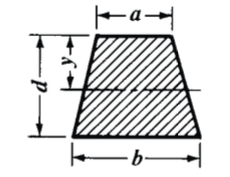
\includegraphics[width=0.3\textwidth]{images/trapecio libro machinery.png}
    \caption{Sección trapezoidal}
    \label{fig:momento_inercia_libro}
\end{figure}



\begin{equation}
    I = \dfrac{ d^3 \cdot (a^2 + 4 \cdot a \cdot b + b^2)}{ 36 (a + b)} \hspace{7pt} (m^4) 
\end{equation}




El momento de inercia generalmente se calcula mediante la posición del centro de masa. Pero las figuras que giran en un eje, no siempre lo hacen con respecto al eje perpendicular que atraviesa el centro de masa, en ocasiones el eje de giro se encuentra fuera de la figura, en ese caso se aplica el $Teorema \text{ } de \text{ } Huygens-Steiner$ o $Teorema \text{ } del \text{ } eje \text{ } paralelo$. \\

Este teorema establece que se puede calcular el momento de inercia de un cuerpo rígido en cualquier eje paralelo al que pasa atravesando a la figura por el centro de masas. Para ello es necesario conocer la distancia perpendicular entre los ejes paralelos (que se definió anteriormente como $brazo$) y la masa del cuerpo, que en nuestro caso será la masa de cada segmento. \\

El teorema de Huygens-Steiner establece lo siguiente:
 \begin{equation}
    I = I_{cm} + m \cdot D^2 \hspace{7pt} (Kg \cdot m^2)
 \label{eq:Huygens-Steiner}
 \end{equation}
 Donde, $I$ := momento de inercia general, $I_{cm}$ := momento de inercia en el centro de masas de un cuerpo rígido, $m$ := masa del cuerpo rígido y $D$ := distancia perpendicular entre los ejes paralelos.\\
 
 

Si se combina la Ecuación \ref{eq:Huygens-Steiner} junto con las variables definidas para el estudio de la pala el momento de inercia vendrá dado por la siguiente definición:
 \begin{equation}
  I_{area} = \dfrac{ L_{i}^3 \cdot (c_{right}^2 + 4 c_{right} \cdot c_{left} + c_{left}^2)}{ 36 (c_{right} + c_{left})} \hspace{7pt} (m^4)
 \label{def:momento_inercia_area}
 \end{equation}
 Donde, $I_{area}$ := momento de inercia de área de una figura de un espesor mínimo para centrar su cálculo en la forma.\\
 
 La anterior ecuación se debe multiplicar por la \textbf{densidad superficial} de la pala del aerogenerador ya que esta representa el momento de inercia de un área, en este caso un trapecio, y se necesita esta densidad para obtener el momento de inercia general.

En el cálculo de la \textbf{densidad superficial} son necesarios dos términos que aún no se han acuñado en este trabajo, la masa y la superficie de una pala. Es cierto que se ha calculado la superficie de los segmentos en la Definición \ref{def:area_segmentos}, ahora solo queda sumarlos.\\


La superficie de la pala es:
 \begin{equation}
 Superficie \text{ } pala = \sum_{i}^{N}s_i \hspace{7pt} (m^2)  
 \label{def:superficie_pala}
 \end{equation}
  Donde, $ Superficie \text{ } pala $ := área de la pala del rotor.\\

En este trabajo solo se han tenido en cuenta los tres materiales mas usados en la construcción de palas de un aerogenerador.\\

Los rangos de densidades de materiales usadas son los siguientes:
 \begin{equation}
 densidad \text{ } pala =  \left\{\begin{matrix}
CFRP = 1500-2000 \hspace{7pt} \left(\dfrac{Kg}{m^3}\right\right)) \cite{MOHAMMED201969}\\\\
GFRP = 910-1200 \hspace{7pt} \left(\dfrac{Kg}{m^3}\right)\right)  \cite{Ephraim2015}\\\\
GF \text{ } Epoxy = 1159-1186 \hspace{7pt} \left(\dfrac{Kg}{m^3}\right) \cite{Tewari2011}
\end{matrix}\right
\label{def:materiales_pala}
\end{equation}
 Donde, $ densidad \text{ } pala $ := densidad de los materiales de los que posiblemente esté compuesta la pala, $ CFRP $ := Carbon fiber reinforced polymer o en castellano; polímero reforzado con fibra de carbono, $ GFRP $ := Glass fiber reinforced polymer o en castellano; polímero reforzado con fibra de vidrio y $GF \text{ } Epoxy $ := Glass fiber reinforced Epoxy o en castellano; Epoxy reforzado con fibra de vidrio.\\

Parte de la pala es hueca. Hay estudios como \textbf{Hollow Blades for Small Wind Turbines Operating at High Altitudes} \cite{Pourrajabian2016}, realizado en 2016, en el que se compara el uso de palas compactas y huecas en determinado escenario y con diferentes grosores de material. \\

En este trabajo, las palas serán huecas y se estima que solo entre un $15-20\%$ de la pala presenta alguno de los materiales que se mencionan. Por ello la expresión de la masa es la siguiente. \\

La masa de los segmentos de una pala dada su densidad y volumen:
 \begin{equation}
 masa \text{ } pala = densidad \text{ } pala \cdot (volumen \text{ } frustum_{total} \cdot (15-20\%) ) \hspace{7pt} (Kg)
 \end{equation}
 \begin{equation}
 masa \text{ } segmento_i = \dfrac{s_i}{superficie \text{ } pala} \cdot masa \text{ } pala \hspace{7pt} (Kg)
 \label{def:masa_pala} 
 \end{equation}
  Donde, $ masa \text{ } pala $ := peso de la aleta de la turbina eólica teniendo en cuenta la porción no rellena de la misma y $ masa \text{ } segmento_i $ := peso de los segmentos de la aleta.\\
 
Se puede pasar a calcular la $densidad \text{ } superficial$ como:
  \begin{equation}
 densidad \text{ } superficial = \dfrac{masa \text{ } pala}{ superficie \text{ } pala} \hspace{7pt} \left(\dfrac{Kg}{m^2}\right)
 \label{def:densidad_superficial}
 \end{equation}
 Donde, $ densidad \text{ } superficial $ := masa de un material por unidad de superficie. \\
 
Se puede obtener el momento de inercia general o $I$, como:
  \begin{equation}
I_{cm} = I_{area} \cdot densidad \text{ } superficial \hspace{7pt} (Kg \cdot m^2)
 \label{def:momento_inercia_cm}
 \end{equation}
 \begin{equation}
I = I_{cm} + masa \text{ } segmento_i \cdot brazo_i^2 \hspace{7pt} (Kg \cdot m^2)
 \label{def:momento_inercia_general}
 \end{equation}

 
\subsection{Velocidad Angular, $\Omega$, en función de la velocidad del viento }

En primer lugar, la velocidad angular, $\Omega$, (Ver Libro \cite[p.~303]{cummings2004understanding}) es "la componente de un vector unidimensional a lo largo del eje de rotación en relación con el sistema de coordenadas elegido para describir el movimiento".\\

Aplicando la anterior definición al sistema que se está estudiando se se tiene que el rotor del aerogenerador sería el eje de rotación en base al cual giran las palas de la turbina. Además el movimiento de giro es constante alrededor del rotor.\\

Una de las opciones más sencillas para el cálculo de la \textit{velocidad angular} es mediante la aceleración angular y la relación que tiene con el \textit{torque} y con el \textit{momento de inercia general}. Pero no era lo suficientemente preciso y no tenía en cuenta todos los aspectos de la cinemática. \\
 
Para que el sistema se encuentre girando a una cierta \textit{velocidad angular} primero se debe producir una cierta \textit{aceleración angular}, producida por el viento. Con el viento y otros factores el rozamiento del aire, el peso de las palas y la fuerza necesaria para moverlas, se podría llegar a mantener una velocidad de giro óptima y así extraer la mayor cantidad de energía. Pero la velocidad del viento es aleatoria, aunque se considera su valor medio como constante.\\


Una de las partes fundamentales es el viento que se presenta delante de la turbina y su velocidad, es decir, la masa o flujo de aire que atravesará el rotor de la turbina. En este caso del aire se obtendrá mediante la relación del volumen frente a la turbina y la densidad del mismo, que puede variar dependiendo de las condiciones meteorológicas.\\

La masa de aire con la que trabaja el rotor es:
\begin{equation}
     diametro \text{ } rotor = 2L + diametro \text{ } gondola \hspace{7pt} (m)
\end{equation}
\begin{equation}
    volumen \text{ } rotor = \dfrac{\pi}{4} \cdot diametro \text{ } rotor^2 \cdot J_{left} \hspace{7pt} (m^3) 
\end{equation}
\begin{equation}
    masa \text{ } aire = volumen \text{ } rotor \cdot \rho \hspace{7pt} (Kg)
\label{def:masa_aire}
\end{equation}
Donde, \textit{diametro rotor} := ancho total del rotor sumando palas y góndola, \textit{diametro gondola} := ancho de la góndola del rotor, \textit{volumen rotor} := tamaño de la figura dibujada (cilindro) por el rotor completo cuando las palas giran y \textit{masa aire} := peso del aire comprendido dentro del volumen del rotor.\\

La energía cinética producida por la masa de aire que comprende el rotor y la velocidad del viento en ese momento es:
\begin{equation}
    energía \text{ } cinética = \dfrac{1}{2} \cdot masa \text{ } aire \cdot u^2 \hspace{7pt} (J)
\end{equation}
Donde, 
    
        $e cinetica = 1/2 * M aire * U VIENTO^2$
        
    Involucramos el coeficiente de potencia con la energía cinética
    
         e cinetica aprovechada = $e cinetica * CP$
         
    Ahora necesitamos la energía cinética de rotación
    
         e cinetica rotacion =$ 1/2 * I * omega^2$

    Se compara y despeja con la energía cinética aprovechada para obtener la velocidad angular omega
    
        $omega = sqrt((CP .* M aire)./I) .* U VIENTO.'$



 \subsection{Potencia de la turbina}
 \label{section:rendimiento}
 
La comparación de potencias da como resultado un rendimiento, este permite determinar si la torsión de la pala genera una variación en la potencia obtenida.\\

El rendimiento del sistema viene definido por:
\begin{equation}
  \eta = \dfrac{potencia \text{ } global_1}{potencia \text{ } global_0}  
 \label{def:rendimiento_potencias}
 \end{equation}
  Donde, $\eta$ := eficiencia respecto a la energía obtenida en dos casos estudiados.\\
 
 Una vez definido el rendimiento, se calcula en base a los resultados obtenidos mediante asignación de valores a variables estándar se pueden dar 3 escenarios:
 

\begin{enumerate}
    \item $\eta < 1$
        \begin{itemize}
            \item En caso de obtener un valor por debajo de 1, quiere decir que la torsión que se aplicó, ha reducido la obtención de energía con respecto al caso base. 
        \end{itemize}
    \item $\eta ~= 1$
        \begin{itemize}
            \item Si el valor obtenido es muy próximo a 1, entonces el caso base y el estudiado proporcionan valores similares de obtención de energía.
        \end{itemize}
    \item $\eta > 1$
        \begin{itemize}
            \item Este es el valor buscado y el objetivo del estudio, que una pala con torsión obtenga más energía que una sin ello.
        \end{itemize}
\end{enumerate}

Cabe recalcar que se deberán hacer numerosas pruebas con diferentes configuraciones de valores .... (SEGUIR)
 
\section{Primeras pruebas en MATLAB}

Desarrollado todo el fundamento teórico detrás del estudio que se está realizando y con el que se está tratando de conocer si mediante torsión de las palas de una turbina eólica se obtiene más energía, menos o la misma que si no se torsionasen, se debe avanzar y comenzar a hacer cálculos empíricos. \\

Estos cálculos y representaciones se realizarán mediante MATLAB, de la manera más ordenada y arbitraria posible. Con esto se busca la manera más simple de poder modificar las variables más sencillas que envuelven a los cálculos, para así poder cambiarlas a placer. \\

Algunas variables como, $L$ y $\Theta_1$ deben ser establecidas por el propio estudiante, dando así un mayor juego a la amplitud de resultados posibles. \\



\section{Conclusiones}

Se diseño una pala simplificada en dos dimensiones en forma de trapezoide y posteriormente se modeló en tres dimensiones. Obteniendo todos los valores necesarios para su inclusión en un estudio numérico mediante el programa MATLAB.\\

Fue realizado el estudio de las fuerzas relacionadas con el viento que afectaban a la pala de un aerogenerador para lograr el cálculo de un torque. Este torque fue definido para cada uno de los N segmentos separados del rotor una distancia basada en la longitud de la pala o radio. También se le aplicó un giro inicial a la pala para poder obtener energía. Esto se debe al mal aerodinamismo de la pala estudiada.\\

El principal elemento de estudio del trabajo se centraba en la torsión. La torsión de la pala es añadida al giro inicial o ángulo de cabeceo en busca de una mayor obtención de energía definida mediante la eficiencia. Se compararon sistemas en los cuales no se presentaba torsión frente a otros que sí, variando los que si tenían. Se obtuvieron resultados mejorados debido a la inclusión de la torsión en los cálculos de las simulaciones.\\

La simulación realizada expone diferentes problemas relacionadas con las hipótesis del diseño de la pala. La pala diseñada e introducida en la simulación se aleja de una manera muy obtusa de una bien diseñada. Otro se relaciona con el grosor de la pala en el borde de fuga cuando la mayoría se achatan, esto no se tuvo en cuenta e indujo a un peor diseño.\\

No se encontraron grandes diferencias entre un ángulo de torsión creciente o decreciente. Requiere estudio para poder determinar si hay alguna que sea mejor que la otra.\\

El número de segmentos también podría influir en una mejora de obtención de energía mediante torsión, requiere mayor profundidad de estudio.


%Bibliografía
\bibliographystyle{unsrt}
\bibliography{biblio}

\end{document}


% Tips:
% -------------------TABLAS -------------------
% Para poner una tabla usa https://www.tablesgenerator.com/
% La haces (o la importas), le das a generate y la pegas en el código
% Le tienes que añadir la H entre los [] para que se coloque bien.

% Ejemplo con la H, el título y la ref:
% \begin{table}[H]
% \begin{tabular}{|c|c|c|c|c|}
% \hline
% as & sd & d & as &   \\ \hline
%   & 1  &   &    & 2 \\ \hline
% 3  & 4  &   &    &   \\ \hline
%   &    &   & 5  &   \\ \hline
% \end{tabular}
% \caption{titulito guay}
% \label{tab:loquesea}
% \end{table}
% Ponle título siempre a las tablas con \caption y siempre que añadas
% una tabla HABLA DE ELLA EN EL TEXTO (en el aptado de FIGURAS te enseño cómo
% se referencian tablas y figuras).
% Recuerda que para poner colorinchis necesitas otra librería
% No me seas cutre y pongas capturas de excel o cosas así como tablas porque te reviento.


%  ------------------- COMENTAR -------------------
% Si quieres comentar un trozaco grande lo seleccionas con el ratón
% y le das crtl + ç y apañao.

%  ------------------- FIGURAS  -------------------
% Referencia SIEMPRE todas las tablas. Es decir, si pones una tabla en
% algún lugar, siempre nómbrala en el texto o te van a echar la bronca.
% Para poner imágenes con caption y poder referenciarlas tienes que utilizar
% la estructura de bloque figure. Te pego un ejemplo aquí y siempre que 
% vayas a necesitar meter una imagen haces copypaste:
% \begin{figure}[H]
%     \centering
%     \includegraphics[width=0.7\textwidth]{images_t11/capas_tcpip.png}
%     \caption{Jerarquía TCP/IP}
%     \label{fig:capas_tcpip}
% \end{figure}
% - El \centering es para centrarlo (hay una forma de ponerlo a la dcha y mas movidas pero no me seas friki y centra las cosas).
% - El include graphics es literalmente para poner la imagen. Déjalas todas
% colocaditas en la carpeta images no me seas disaster y si tienes muchas
% puedes incluso crear más carpetas, pero recuerda cambiar el include.
% En el width como puedes imaginar puedes cambiarle el tamaño, en el ejemplo es 0.7
% ni idea de qué medida usa, a veces es cm a veces pixeles, vas probando y ya.
% - El caption es el título que le pones
% - Label es la etiqueta que le pones a la imagen para poder referenciarla.
% A las figuras siempre ponle fig:loquesea, y a las tablas, que también le
% tienes que poner siempre referencias, le pones tab:loquesea. Luego en el texto,
% para referenciar esa figura o tabla usa el comando \ref. Por ejemplo "Como podemos observar
% en la \ref{tab:loquesea}..." y te va a aparecer en el pdf:  "Como podemos observar
% en la Tabla 1"
% Le puedes añadir además texto a la tabla como para describirla si te hace falta, 
% eso lo pones a piñón en la siguiente línea después de \label y queda bien.
% Puedes hacer subfigures en plan dos figuras dentro de una figura para poder
% referenciarlas juntas o por separado. Por ejemplo poder tener: Figura 1, Figura 1a y Figura 1b
% pero es un lío, tengo por ahí algún ejemplo, si lo necesitas lo busco.

% ------------------- NEGRITAS CURSIVAS ---------------------
% Se pueden usar negritas y cursivas, le das ctrl b y ctrl i y tirando

% ------------------- LISTADO ---------------------
% Para hacer un listado tienes que utilizar el bloque itemize o el enumerate
% Ejemplo:
% \begin{enumerate}
%     \item pito
%     \item nepe
% \end{enumerate}
% o
% \begin{itemize}
%     \item hola
% \end{itemize}
% La diferencia es que enumerate es enumerado e itemice son puntitos.
% Si abres otro itemize dentro de uno se te crean subpuntos
% Si te motivas o no te gustan los puntitos hay comandos para poner guiones, circunferencias
% o cualquier símbolo

% --------------- FÓRMULAS MATES ----------------
% De fórmulas matemáticas tengo 3000 ejemplos, pregúntame si no sabes.
% Lo importante que sepas que para ponerlas centradas se usa doble dolar: $$ fórmula $$
% y para ponerlas siguiendo al texto solo un dolar: $ formula $
% igual te digo, no pongas capturas de fórmulas, hazlas aquí.
% Si quieres poner un símbolo en plan epsilon, beta, omega, ro, te vas a google y lo buscas,
% no deberías tener problemas porque te he añadido el paquete que se necesita.

% --------------- CUADRITOS CHULIS ----------------
% Te he añadido otra kkita que se llama mdframed
% que es para encuadrar algún textito así para que quede como destacado,
% se suele utilizar para teoremas, definiciones, corolarios...
% https://tools.ietf.org/doc/texlive-doc/latex/mdframed/mdframed-example-default.pdf
% A mí me gusta pero haz lo que veas. Se le puede añadir título, colores...

% \mdfdefinestyle{theoremstyle}{%
% linecolor=blue!40,linewidth=2pt,%
% frametitlerule=true,%
% frametitlebackgroundcolor=gray!20,
% innertopmargin=\topskip,
% }
% \mdtheorem[style=theoremstyle]{definition}{Definition}
% \begin{definition}[Me gusta esto]
% \ExampleText
% \end{definition}


% --------------- CÓDIGO ----------------
% Vas a hacer código matlab 100% entonces para añadir código aquí y que quede tope guapo
% hay otra librería con la que puedes hacer un cuadrito como el de mdframed pero
% para algoritmos y le pones el lenguaje que es y te lo pone a color
% siguiendo la sintaxis de ese lenguaje.
% No me acuerdo cómo se llamaba pero te lo busco cuando lo necesites, babe.


% --------------- LA MAGIA DE LAS COMILLAS ----------------
% Si quieres citar algo, en español sabes que se usa " ", pero como esto es latex
% y son yankis que citan con ' ' pues alv, no funcionan nuestras comas.
% Tienes que usar `` '', es decir, dos veces la tilde francesa que está al lado de la p en el teclado para abrir comillas y dos veces la comilla simple de donde la interrogación para cerrar.
% Por ejemplo: Como dijo Perico el de los Palotes \cite{perico1990palotes} ``Santa Rita
% Rita lo que se da no se quita''
% Te he colado arriba un cite para que ya te sirva de ejemplo de eso también.
% Btw los alemanes citan con „ " ¿qué les pasa? eso ya no sé cómo se pone en latex sorry.

% Posdata: tk
